\documentclass{standalone}
\usepackage{tikz}
\usetikzlibrary{patterns, positioning}


\begin{document}
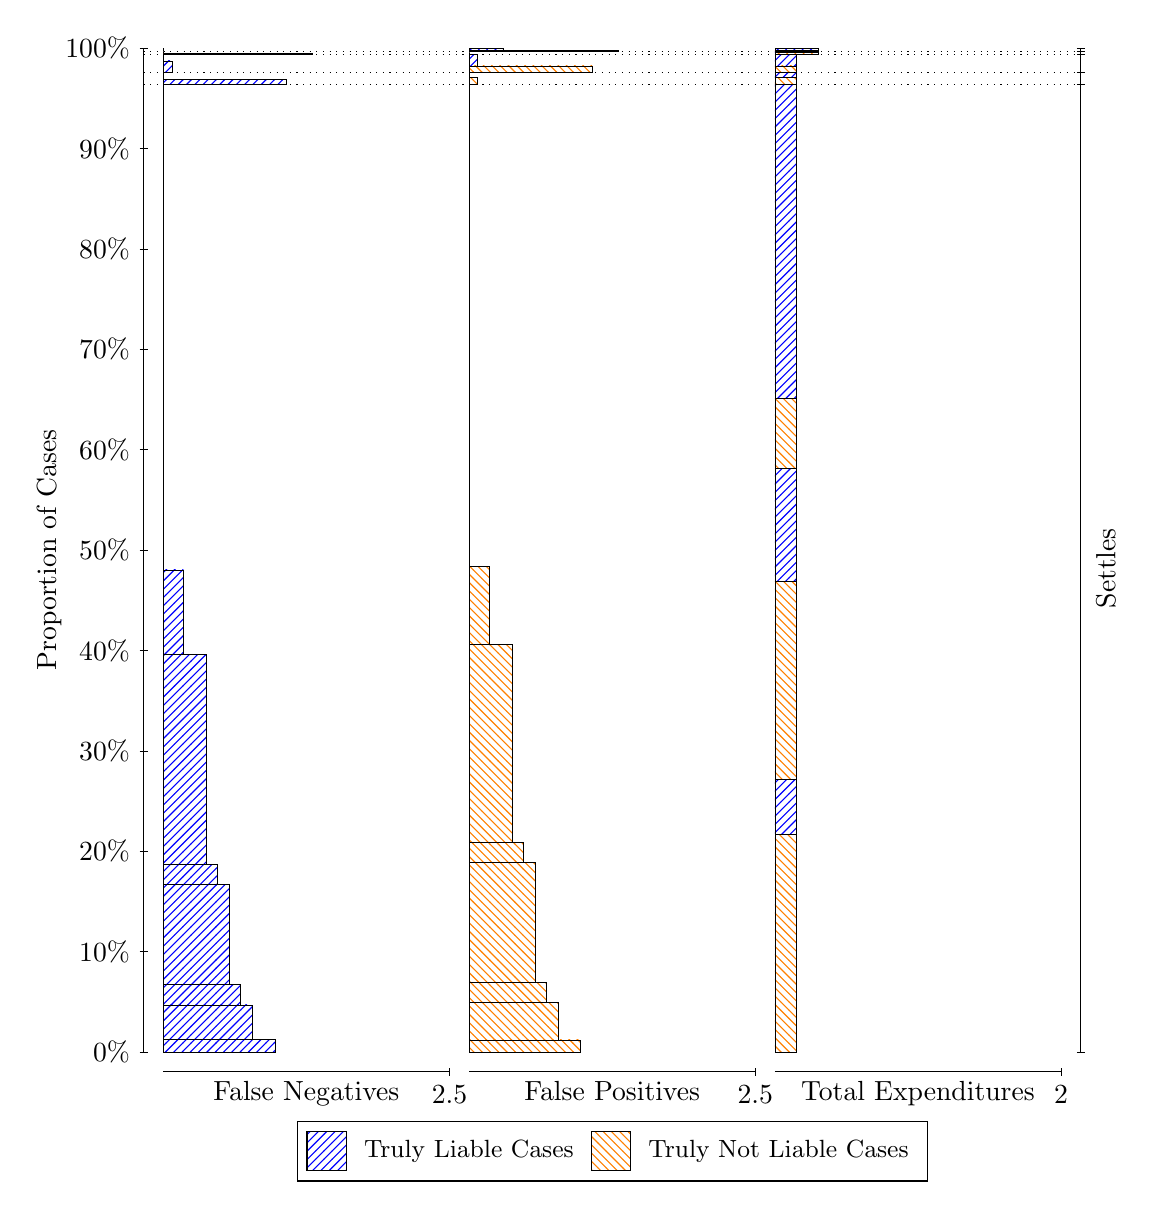
\begin{tikzpicture}
\draw[black, very thin] (1.5,1.75) -- (1.5,14.5);
\node[rotate=90, text=black, anchor=center] at (0.3, 8.125) {Proportion of Cases};
\draw[black, very thin] (1.45,1.75) -- (1.55,1.75);
\node[text=black, anchor=east] at (1.45, 1.75) {0\%};
\draw[black, very thin] (1.45,3.025) -- (1.55,3.025);
\node[text=black, anchor=east] at (1.45, 3.025) {10\%};
\draw[black, very thin] (1.45,4.3) -- (1.55,4.3);
\node[text=black, anchor=east] at (1.45, 4.3) {20\%};
\draw[black, very thin] (1.45,5.575) -- (1.55,5.575);
\node[text=black, anchor=east] at (1.45, 5.575) {30\%};
\draw[black, very thin] (1.45,6.85) -- (1.55,6.85);
\node[text=black, anchor=east] at (1.45, 6.85) {40\%};
\draw[black, very thin] (1.45,8.125) -- (1.55,8.125);
\node[text=black, anchor=east] at (1.45, 8.125) {50\%};
\draw[black, very thin] (1.45,9.4) -- (1.55,9.4);
\node[text=black, anchor=east] at (1.45, 9.4) {60\%};
\draw[black, very thin] (1.45,10.675) -- (1.55,10.675);
\node[text=black, anchor=east] at (1.45, 10.675) {70\%};
\draw[black, very thin] (1.45,11.95) -- (1.55,11.95);
\node[text=black, anchor=east] at (1.45, 11.95) {80\%};
\draw[black, very thin] (1.45,13.225) -- (1.55,13.225);
\node[text=black, anchor=east] at (1.45, 13.225) {90\%};
\draw[black, very thin] (1.45,14.5) -- (1.55,14.5);
\node[text=black, anchor=east] at (1.45, 14.5) {100\%};

\draw[black, very thin] (13.4,1.75) -- (13.4,14.5);
\draw[black, very thin] (13.35,1.75) -- (13.45,1.75);
\node[anchor=west] at (13.35, 1.75) {};
\draw[black, very thin] (13.35,14.039) -- (13.45,14.039);
\node[anchor=west] at (13.35, 14.039) {};
\draw[black, very thin] (13.35,14.19) -- (13.45,14.19);
\node[anchor=west] at (13.35, 14.19) {};
\draw[black, very thin] (13.35,14.419) -- (13.45,14.419);
\node[anchor=west] at (13.35, 14.419) {};
\draw[black, very thin] (13.35,14.459) -- (13.45,14.459);
\node[anchor=west] at (13.35, 14.459) {};
\draw[black, very thin] (13.35,14.5) -- (13.45,14.5);
\node[anchor=west] at (13.35, 14.5) {};

\draw[black, very thin, pattern color=blue, pattern=north east lines] (1.75,1.75) rectangle (3.167,1.9088);
\draw[black, very thin, pattern color=blue, pattern=north east lines] (1.75,1.9088) rectangle (2.8763,2.3485);
\draw[black, very thin, pattern color=blue, pattern=north east lines] (1.75,2.3485) rectangle (2.731,2.6042);
\draw[black, very thin, pattern color=blue, pattern=north east lines] (1.75,2.6042) rectangle (2.5857,3.8789);
\draw[black, very thin, pattern color=blue, pattern=north east lines] (1.75,3.8789) rectangle (2.4403,4.1346);
\draw[black, very thin, pattern color=blue, pattern=north east lines] (1.75,4.1346) rectangle (2.295,6.7949);
\draw[black, very thin, pattern color=blue, pattern=north east lines] (1.75,6.7949) rectangle (2.0043,7.8717);
\draw[black, very thin, pattern color=orange, pattern=north west lines] (1.75,7.8717) rectangle (1.75,14.039);
\draw[black, very thin, pattern color=blue, pattern=north east lines] (1.75,14.039) rectangle (3.3123,14.105);
\draw[black, very thin, pattern color=orange, pattern=north west lines] (1.75,14.105) rectangle (1.75,14.19);
\draw[black, very thin, pattern color=blue, pattern=north east lines] (1.75,14.19) rectangle (1.859,14.336);
\draw[black, very thin, pattern color=orange, pattern=north west lines] (1.75,14.336) rectangle (1.75,14.419);
\draw[black, very thin, pattern color=blue, pattern=north east lines] (1.75,14.419) rectangle (3.6393,14.433);
\draw[black, very thin, pattern color=orange, pattern=north west lines] (1.75,14.433) rectangle (1.75,14.459);
\draw[black, very thin, pattern color=orange, pattern=north west lines] (1.75,14.459) rectangle (1.75,14.473);
\draw[black, very thin, pattern color=blue, pattern=north east lines] (1.75,14.473) rectangle (1.75,14.5);
\draw[black, very thin, pattern color=orange, pattern=north west lines] (5.6333,1.75) rectangle (7.0503,1.9031);
\draw[black, very thin, pattern color=orange, pattern=north west lines] (5.6333,1.9031) rectangle (6.7597,2.3818);
\draw[black, very thin, pattern color=orange, pattern=north west lines] (5.6333,2.3818) rectangle (6.6143,2.6374);
\draw[black, very thin, pattern color=orange, pattern=north west lines] (5.6333,2.6374) rectangle (6.469,4.1591);
\draw[black, very thin, pattern color=orange, pattern=north west lines] (5.6333,4.1591) rectangle (6.3237,4.4148);
\draw[black, very thin, pattern color=orange, pattern=north west lines] (5.6333,4.4148) rectangle (6.1783,6.9255);
\draw[black, very thin, pattern color=orange, pattern=north west lines] (5.6333,6.9255) rectangle (5.8877,7.9172);
\draw[black, very thin, pattern color=blue, pattern=north east lines] (5.6333,7.9172) rectangle (5.6333,14.039);
\draw[black, very thin, pattern color=orange, pattern=north west lines] (5.6333,14.039) rectangle (5.7423,14.124);
\draw[black, very thin, pattern color=blue, pattern=north east lines] (5.6333,14.124) rectangle (5.6333,14.19);
\draw[black, very thin, pattern color=orange, pattern=north west lines] (5.6333,14.19) rectangle (7.1957,14.273);
\draw[black, very thin, pattern color=blue, pattern=north east lines] (5.6333,14.273) rectangle (5.7423,14.419);
\draw[black, very thin, pattern color=orange, pattern=north west lines] (5.6333,14.419) rectangle (5.6333,14.446);
\draw[black, very thin, pattern color=blue, pattern=north east lines] (5.6333,14.446) rectangle (5.6333,14.459);
\draw[black, very thin, pattern color=orange, pattern=north west lines] (5.6333,14.459) rectangle (7.5227,14.473);
\draw[black, very thin, pattern color=blue, pattern=north east lines] (5.6333,14.473) rectangle (6.0693,14.5);
\draw[black, very thin, pattern color=orange, pattern=north west lines] (9.5167,1.75) rectangle (9.7892,4.5164);
\draw[black, very thin, pattern color=blue, pattern=north east lines] (9.5167,4.5164) rectangle (9.7892,5.2118);
\draw[black, very thin, pattern color=orange, pattern=north west lines] (9.5167,5.2118) rectangle (9.7892,7.7252);
\draw[black, very thin, pattern color=blue, pattern=north east lines] (9.5167,7.7252) rectangle (9.7892,9.1587);
\draw[black, very thin, pattern color=orange, pattern=north west lines] (9.5167,9.1587) rectangle (9.7892,10.046);
\draw[black, very thin, pattern color=blue, pattern=north east lines] (9.5167,10.046) rectangle (9.7892,14.039);
\draw[black, very thin, pattern color=orange, pattern=north west lines] (9.5167,14.039) rectangle (9.7892,14.124);
\draw[black, very thin, pattern color=blue, pattern=north east lines] (9.5167,14.124) rectangle (9.7892,14.19);
\draw[black, very thin, pattern color=orange, pattern=north west lines] (9.5167,14.19) rectangle (9.7892,14.273);
\draw[black, very thin, pattern color=blue, pattern=north east lines] (9.5167,14.273) rectangle (9.7892,14.419);
\draw[black, very thin, pattern color=orange, pattern=north west lines] (9.5167,14.419) rectangle (10.062,14.446);
\draw[black, very thin, pattern color=blue, pattern=north east lines] (9.5167,14.446) rectangle (10.062,14.459);
\draw[black, very thin, pattern color=orange, pattern=north west lines] (9.5167,14.459) rectangle (10.062,14.473);
\draw[black, very thin, pattern color=blue, pattern=north east lines] (9.5167,14.473) rectangle (10.062,14.5);
\draw[black, dotted] (1.5,14.039) -- (13.4,14.039);
\draw[black, dotted] (1.5,14.19) -- (13.4,14.19);
\draw[black, dotted] (1.5,14.419) -- (13.4,14.419);
\draw[black, dotted] (1.5,14.459) -- (13.4,14.459);
\draw[black, very thin] (1.75,1.5) -- (5.3833,1.5);
\node[text=black, anchor=north] at (3.5667, 1.5) {False Negatives};
\draw[black, very thin] (5.3833,1.45) -- (5.3833,1.55);
\node[text=black, anchor=north] at (5.3833, 1.45) {2.5};

\draw[black, very thin] (5.6333,1.5) -- (9.2667,1.5);
\node[text=black, anchor=north] at (7.45, 1.5) {False Positives};
\draw[black, very thin] (9.2667,1.45) -- (9.2667,1.55);
\node[text=black, anchor=north] at (9.2667, 1.45) {2.5};

\draw[black, very thin] (9.5167,1.5) -- (13.15,1.5);
\node[text=black, anchor=north] at (11.333, 1.5) {Total Expenditures};
\draw[black, very thin] (13.15,1.45) -- (13.15,1.55);
\node[text=black, anchor=north] at (13.15, 1.45) {2};

\node[text=black, centered, rotate=90] at (13.72, 7.8944) {Settles};





\draw (7.449999999999999,1.5) node[draw=none] (baseCoordinate) {};
\begin{scope}[align=center]
        \matrix[scale=0.5, draw=black, below=0.5cm of baseCoordinate, nodes={draw}, column sep=0.1cm]{
            \node[rectangle, draw, minimum width=0.5cm, minimum height=0.5cm, pattern color=blue, pattern=north east lines] {}; &
            \node[draw=none, font=\small, text=black] (B) {Truly Liable Cases}; &
            \node[rectangle, draw, minimum width=0.5cm, minimum height=0.5cm, pattern color=orange, pattern=north west lines] {}; &
            \node[draw=none, font=\small, text=black] (B) {Truly Not Liable Cases}; \\
            };
\end{scope}

\end{tikzpicture}
\end{document}